% Inkludieren benötigter Packages
% ===============================
\documentclass[liststotoc, bibtotoc, pointlessnumbers, a4paper,
12pt]{scrreport}
% benötigte Packages für deutsche Texte
\usepackage[ngerman]{babel} % Deutsche Einstellungen
\usepackage[utf8]{inputenc} % utf-8 Eingabe
\usepackage[T1]{fontenc}
\usepackage{csquotes}

% Packages für mathemaische Formelsätze
\usepackage{amsmath}
\usepackage{amssymb}
\usepackage{fleqn}
\setlength{\mathindent}{1cm}

% Packages zum Einbinden von Bildern
\usepackage{graphicx}
\usepackage{float}

% Package für Tabellenumgebung
\usepackage{booktabs}

% Packages zum Einlesen von Scilab-Code
\usepackage{listings}
\usepackage{xcolor}

\definecolor{codegreen}{rgb}{0,0.6,0}
\definecolor{codegray}{rgb}{0.5,0.5,0.5}
\definecolor{codepurple}{rgb}{0.58,0,0.82}
\definecolor{backcolour}{rgb}{0.95,0.95,0.92}

\lstdefinestyle{mystyle}{
	backgroundcolor = \color{backcolour},   
	commentstyle = \color{codegreen},
	keywordstyle = \color{magenta},
	numberstyle = \tiny\color{codegray},
	stringstyle = \color{codepurple},
	basicstyle = \ttfamily\scriptsize,
	breakatwhitespace = false,         
	breaklines = true,                 
	captionpos = b,                    
	keepspaces = true,                 
	numbers = left,                    
	numbersep = 5pt,                  
	showspaces = false,                
	showstringspaces = false,
	showtabs = false,                  
	tabsize = 2
}

\lstset{literate=%
	{Ö}{{\"O}}1
	{Ä}{{\"A}}1
	{Ü}{{\"U}}1
	{ß}{{\ss}}1
	{ü}{{\"u}}1
	{ä}{{\"a}}1
	{ö}{{\"o}}1
}

\lstset{style=mystyle}

% Packages für die Zitation
\usepackage[backend = bibtex,
style = numeric,
bibstyle = numeric,
citestyle = numeric,
natbib = false,
mcite = false,
maxcitenames = 3,
sorting = nyt]{biblatex}
\addbibresource{Bibliography.bib}

% Will man die Bilder aus einem eigenen Ordner aufrufen -> Pfad muss angegeben werden
\graphicspath{{Bilder/}}

% Definieren des Aufzählungssymbols
\def\labelitemi{--}

%==============================================================================
% 							  Hauptdokument
%==============================================================================

\begin{document}
	% Titelblatt und Inhaltsverzeichnis
	% ---------------------------------
	\begin{titlepage}
		\centering
		
\includegraphics[width=0.7\textwidth]{FH.png}\par
		\vspace{2.5cm}
		\Huge\textbf{PRT3LB: Modellflugzeug}\par
		\vspace{1cm}
		\hrule
		\vspace{2cm}
		\begin{center}
			\begin{tabular}{ll}
				\large Darius Faje			&	\large S2310566006	\\
				\large Erik Großhaupt		&	\large S2310566008	\\
			\end{tabular}
		\end{center}\par
		%
		\vspace{2 cm}
		%
		\large\today\par
		\large FH-OÖ Campus Wels \par
		\large MB.ma \par
	\end{titlepage}
	%
	\newpage
	%
	\tableofcontents
	%
	\newpage
	%--------------------------------------------------------------------------
%%----------------------------------------------------------------------------
	\clearpage
%%----------------------------------------------------------------------------
%% Einleitung	
	\chapter{Aufgabenstellung}
\label{sec: Einleitung}

% Allgemeine Aufgabenstellung
%----------------------------
Im Zuge dieser Laborübung soll ein Modellflugzeug schwingungstechnisch untersucht
werden. Dabei gilt es, 4 verschiedene Aufgabenstellungen abzuhandeln. Um die
Leserlichkeit zu erleichtern, werden die einzelnen Aufgabenstellung in eigenen
Unterkapiteln jeweils vollständig abgearbeitet.

%%----------------------------------------------------------------------------
%% Hauptkapitel 1
	\chapter{Experimentelle Modalanalyse des Modellflugzeugs}
\label{sec: Hauptkapitel 1}

\section{Aufgabenstellung}
%=========================
    % Grundsätzliches Ziel
    %---------------------
    Bei dieser Laboraufgabe sollen die tieffrequenten Schwingungsmoden des
    Modellflugzeugs bestimmt werden. Die Bestimmung der Moden soll mittels
    experimenteller Modalanalyse durchgeführt werden.
    \\
    %----------------------------------------------------------------------------

    % Ausdetaillierung
    %-----------------
    \noindent
    Es soll dabei bei der Bestimmung der Übertragungsfunktionen kein fertiger
    FRF-Block von Labview verwendet werden. Stattdessen sollen die
    Übertragungsfunktionen durch Division des gemessenen Ausgangs- durch
    Eingangssignals bestimmt werden.
%================================================================================

\section{Versuchsaufbau}
%=======================
    % Diskretisierung des Fliegers
    %-----------------------------
    Da die Messung nur an jeweils einzelnen Punkten durchgeführt werden kann,
    wird in einem ersten Schritt der Modllflieger diskretisiert. Die Messpunkte
    werden dabei mittels Klebenband gekennzeichnet und über Nummern
    unterschieden. Bei der Diskretisierung wird das Modellflugzeug in 3 Bereiche
    unterteilt.
    %----------------------------------------------------------------------------

    % Tab. - Diskretisierung
    %-----------------------
    \begin{table}[h]
        \centering
        \begin{tabular}{|l|c|c|}
            \hline
            \textbf{Bereich} &   \textbf{Schriftfarbe}    &   \textbf{Anzahl der Messpunkte}   \\
            \hline \hline
            vorderer Tragflügel &   rot &   5   \\
            \hline
            Rumpf   &   grün    &   3   \\
            \hline
            hintere Flosse  &   blau    &   2   \\
            \hline
        \end{tabular}
        \caption{Diskretisierung des Modellflugzeugs}
        \label{tab: Fliegerdiskretisierung}
    \end{table}
    %----------------------------------------------------------------------------

    \noindent
    Das diskretisierte Modellflugzeug ist in Abbildung
    \ref{fig: Flieger_diskretisiert} zu sehen.

    % Bild - Diskretisiertes Modellflugzeug
    %--------------------------------------
    \begin{figure}[H]
        \centering
        \includegraphics[width=0.95\textwidth]{Flieger_diskretisiert_Comp.png}
        \caption{diskretisiertes Modellflugzeug}
        \label{fig: Flieger_diskretisiert}
    \end{figure}

    % Bildbeschreibung
    %-----------------
    \noindent
    In Abbildung \ref{fig: Flieger_diskretisiert} sind nur 2 grün beschriftete
    Messpunkte für den Rumpf zu sehen. Das liegt daran, dass der rot markierte
    Punkt 3 des vorderen Tragflügels auch für die Rumpfmessungen herangezogen
    wird.
    \\
    %----------------------------------------------------------------------------

    % Versuchsdurchführung
    %---------------------
    \noindent
    Um die tieffrequenten Moden des Fliegers zu bestimmen, muss in einem ersten
    Schritt die Übertragungsfunktionenmatrix bestimmt werden. Dazu werden
    Messungen mit dem Impulshammer durchgeführt, bei denen ein
    Beschleunigungssignal aufgenommen wird. Es wird dabei die Methode Roving
    Hammer verwendet. Der Beschleunigungssensor bleibt somit immer an Position
    \glqq 5 rot\grqq \hspace{0.05cm} am vorderen Tragflügel (siehe Abbildung
    \ref{fig: Flieger_diskretisiert}).
    %----------------------------------------------------------------------------

    % Verwendete Geräte
    %------------------
    \noindent
    Die verwendeten Messgeräte sind in Tabelle \ref{tab: Geräteliste_EMA}
    angeführt.

    \begin{table}[H]
        \centering
        \begin{tabular}{|l|l|l|}
            \hline
            \textbf{Gerät}  &   \textbf{Seriennummer}   &   \textbf{Sensordaten} \\
            \hline \hline
            Beschleunigungssensor & ... & ... \\
            \hline
            Impulshammer & ... & ... \\
            \hline
            Messkarte & ... & ... \\
            \hline
        \end{tabular}
        \caption{Geräteliste - Experimentelle Modalanalyse}
        \label{tab: Geräteliste_EMA}
    \end{table}    
%================================================================================

\section{Ergebnisse}
%===================
    % Berechnen der Übertragungsfunktion
    %-----------------------------------
    Die Berechnung der Übertragungsfunktionen erfolgt über ein Python-Skript.
    Dieses liest die Messergebnisse, die mit Labview in ein  Excelfile
    gespeichert wurden ein, transformiert diese in den Frequenzbereich und
    bestimmt dann die Übertragungsfunktion. Anschließend werden die Ergebnisse
    wieder in ein Excelfile rausgeschrieben.
    \\
    %----------------------------------------------------------------------------

    % Bestimmen der Moden
    %--------------------
    \noindent
    Die Moden des Flugzeugs können nun durch Betrachtung der
    Übertragungsfunktionen bestimmt werden. Um die Frequenzlage zu bestimmen,
    wird der Bereich, in dem im Plot der Übertragungsfunktionen ein Mode
    vermutetet wird, genauer betrachtet. Im Falle der Amplitude wird ein
    Maximum in diesem Bereich gesucht. Bei Betrachtung des Imaginärteils wird der
    größte Absolutwert im Bereich verwendet und bei Betrachtung des Realteils
    wird ein Nulldurchgang gesucht. Dieser Vorgang wird für jede
    Übertragungsfunktion durchgeführt. Die sich dadurch ergebenden
    Frequenzlagen werden zu einem Mittelwert zusammengefasst. Somit ergeben sich
    3 gemittelte Frequenzlagen der Moden, einmal aus der Amplitude, einmal aus 
    dem Imaginärteil und aus dem Realteil. Im Anschluss werden diese 3
    Mittelwerte erneut zu einem Mittelwert zusammengefasst. Es ergeben sich
    folgende, tieffrequente Moden des Modellflugzeugs:
    %----------------------------------------------------------------------------

    % Tabelle mit den Moden
    %----------------------
    \begin{table}[H]
        \centering
        \begin{tabular}{|c|c|}
            \hline
            \textbf{Mode}   &   \textbf{Frequenzlage [Hz]}  \\
            \hline \hline
            Mode 1  &   5.048 \\
            \hline
            Mode 2  &   20.02 \\
            \hline
            Mode 3  &   46.34 \\
            \hline
            Mode 4  &   49.707 \\
            \hline            
        \end{tabular}
        \caption{Frequenzlage der tieffrequenten Moden}
        \label{tab: Frequenzlage_Moden}
    \end{table}
    %----------------------------------------------------------------------------

    % Amplitudenplot
    %---------------
    \noindent
    Diese 4 Moden decken sich auch gut mit den Betrachtungen des Plots der
    Amplituden der Übertragungsfunktionen (siehe Abbildung
    \ref{fig: Amplitudenplot}).

    % Bild - Amplitudenplot
    %----------------------
    \begin{figure}[H]
        \centering
        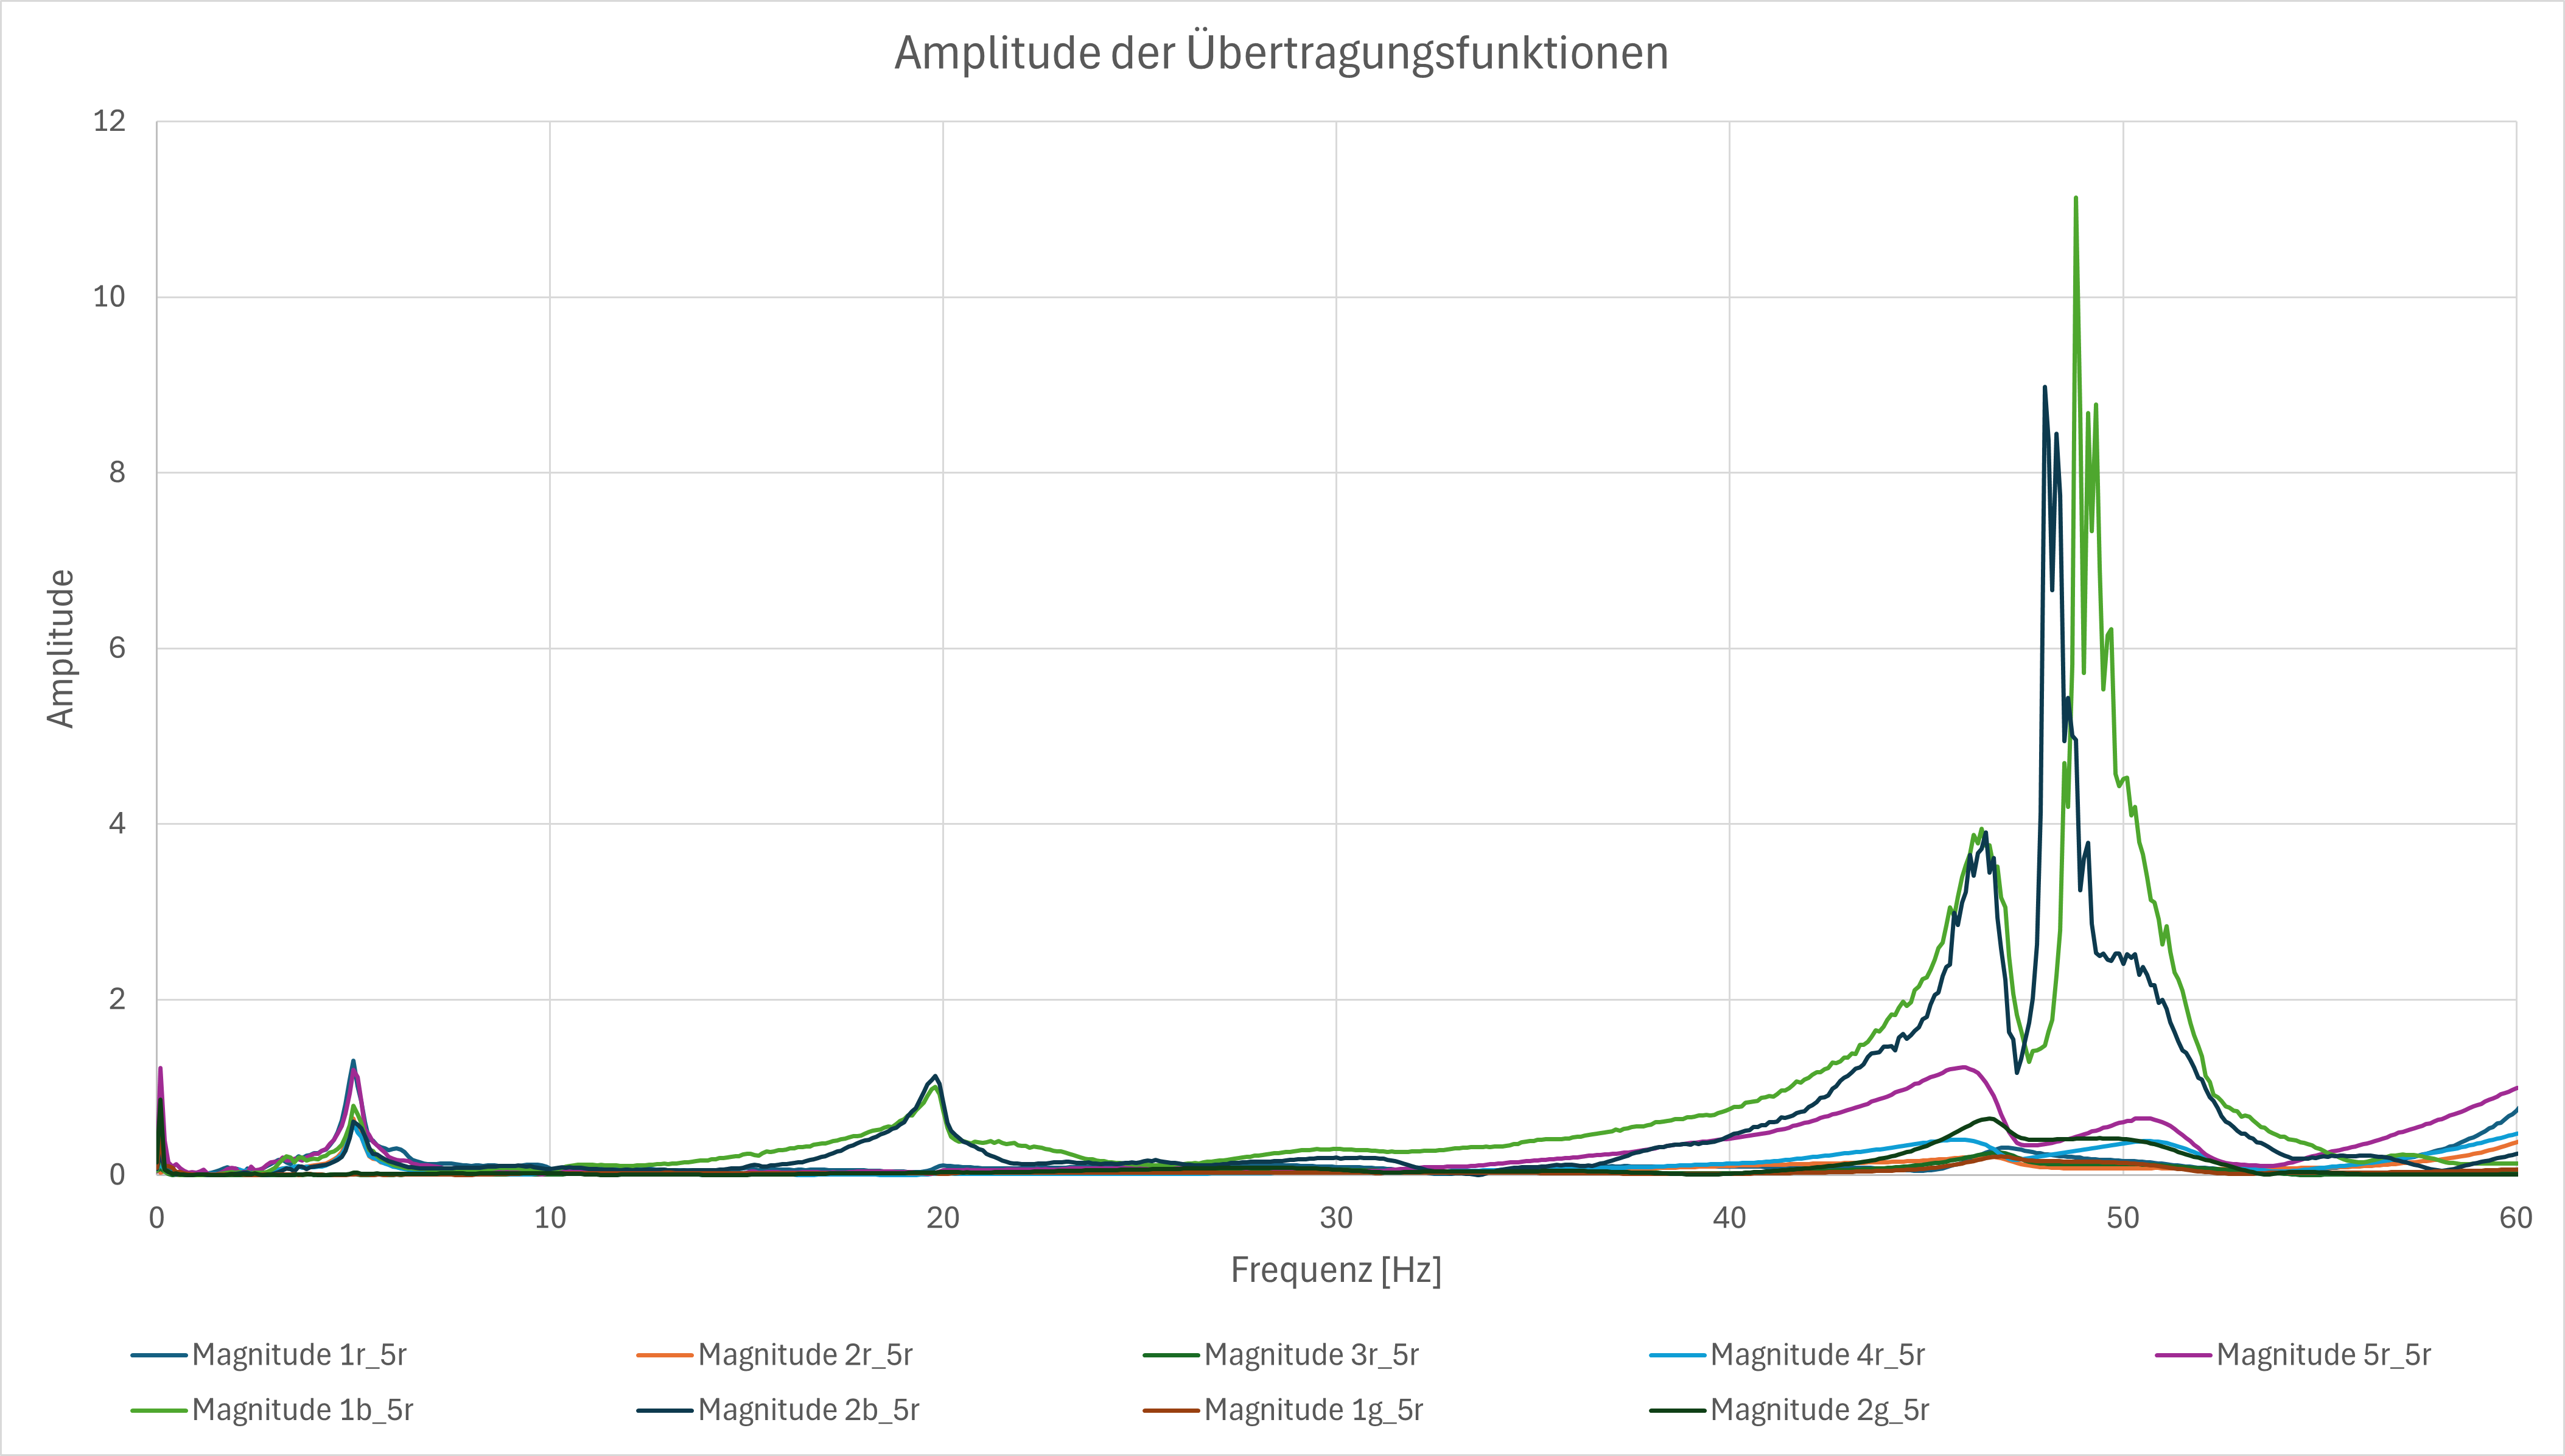
\includegraphics[width=0.95\textwidth]{Amplitudenplot.png}
        \caption{Amplitude der Übertragungsfunktionen}
        \label{fig: Amplitudenplot}
    \end{figure}
    %----------------------------------------------------------------------------

    % 
%%----------------------------------------------------------------------------
%% Hauptkapitel 2
	\chapter{Betriebsschwingungsanalyse}
\label{sec: Hauptkapitel 2}


\section{Aufgabenstellung}
%=========================
    % Grundziel
    %----------
    Ziel dieser Laboraufgabe ist das Durchführen einer Betriebsschwingungsanalyse
    mit anschließender Erstellung eines Campbell-Diagramms. Der Motor des
    Modellflugzeugs soll dabei von einem Elektromotor ohne Verdichtung
    geschleppt werden. Das Schwingungssignal soll an einem bestimmten Punkt der
    Tragfläche abgenommen werden.
%================================================================================

\section{Versuchsaufbau}
%=======================
    % Verwendete Geräte
    %------------------
    Für diesen Versuchsaufbau wurden folgende Geräte verwendet:

    \begin{table}[H]
        \centering
        \begin{tabular}{|l|l|p{6cm}|}
            \hline
            \textbf{Gerät}  &   \textbf{Gerätename}   &   \textbf{Sensordaten} \\
            \hline \hline
            CompaqDAQ Chassis & cDAQ-9171 & hostpowered \\
            \hline
            CompaqDAQ Input Modul & NI 9234 & 4 Kanäle, ±5 V, 51,2 kS/s pro Kanal, 24 bit-IEPE  \\
            \hline
            CompaqDAQ Output Modul & NI 9201 & 8 Kanälen, 500 kS/s, 12 bit, ±10 V   \\
            \hline
            Beschleunigungssensor & 8702B25 & Kistler, Piezo, ±25g, 1Hz-9kHz, UniAx, 169 mV/g  \\
            \hline
            Beschleunigungssensor & 8702B25 & Kistler, Piezo, ±50g, 0.5Hz-5kHz, UniAx, 96.5 mV/g  \\
            \hline
            Elektromotor & - & FH-Wels, max. 12 V \\
            \hline
        \end{tabular}
        \caption{Geräteliste - Betriebsschwingungsanalyse}
        \label{tab: Geräteliste_BSA}
    \end{table}

    % Sensorplatzierung
    %------------------
    \noindent
    Obwohl nur ein Sensorsignal ausgewertet werden muss, werden 4
    Beschleunigungssensoren am vorderen Tragflügel positioniert platziert.
    Somit kann mit einem Aufbau und einer Messung sowohl die Aufgabe von Kapitel
    \ref{sec: Hauptkapitel 2} und Kaptiel \ref{sec: Hauptkapitel 3}
    abgewickelt werden. Die Beschleunigungssensoren werden an Punkten 1, 2, 4 und
    5 rot platziert (siehe Abbildung \ref{fig: Sensorpos_BSA}). Im Zuge von
    Kapitel \ref{sec: Hauptkapitel 2} wird der Messpunkt 5 rot verwendet und in
    weiterer Folge als Messpunkt 1 bezeichnet.

    % Bild - Sensorplatzierung BSA
    %-----------------------------
    \begin{figure}[H]
        \centering
        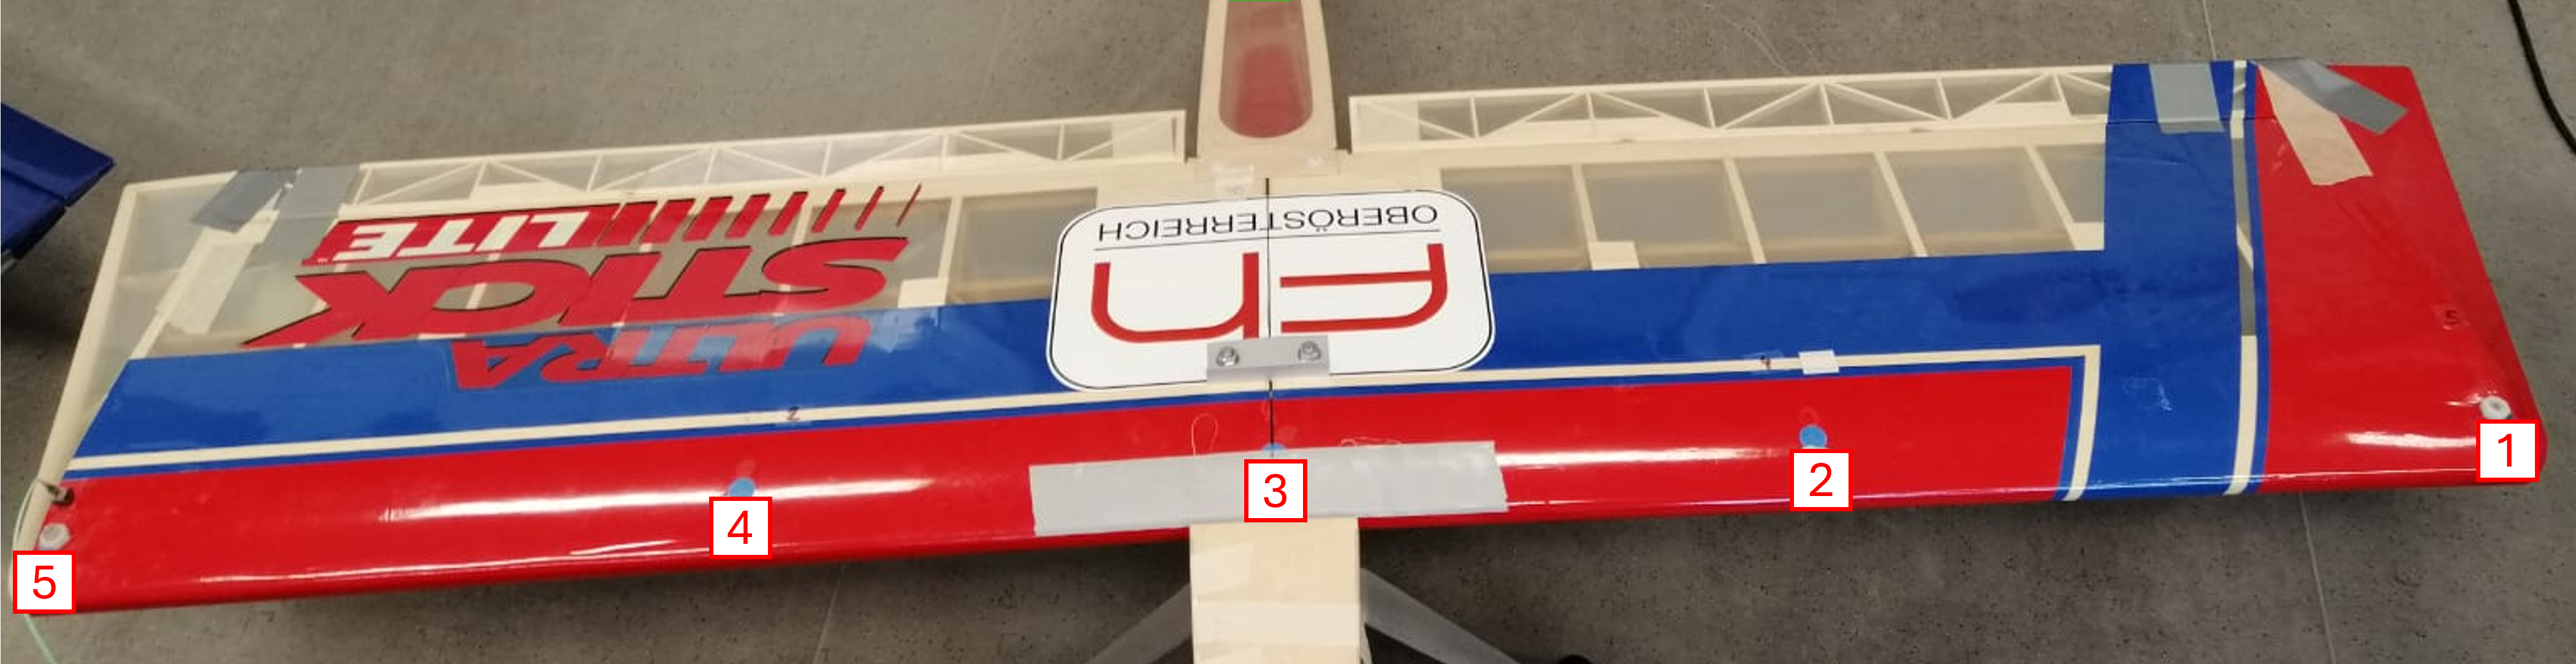
\includegraphics[width=0.9\textwidth]{BSA_Sensorpositionen.png}
        \caption{Sensorpositionen BSA}
        \label{fig: Sensorpos_BSA}
    \end{figure}
    %----------------------------------------------------------------------------

    % Fixierung Flieger
    %------------------
    \noindent
    Damit der Modellflieger bei den Messungen nicht durch die Schwingungen
    verfahren wird, wird er am Boden fixiert. Dazu werden behelfsmäßige Keile mit
    Klebeband am Boden bei den Rädern befestigt.
    \\
    %----------------------------------------------------------------------------

    % Messung mit Motor
    %------------------
    \noindent
    Bevor nun die Betriebsschwingungsanalyse durchgeführt werden kann, wird der
    Motor des Modellflugzeugs mit etwas Öl geschmiert. Dann wird der Elektromotor
    an die Welle zum Übertragen des Drehmoments angesetzt. Nun kann die Messung
    gestartet werden. Dabei wird der Elektromotor langsam mit einer Rampe von einer
    Spannung von 0 [V] auf 5 [V] beschleunigt. Während der Messung wird der
    Elektromotor in der Hand gehalten.
    %----------------------------------------------------------------------------

    % Drehzahlmessung
    %----------------
    \noindent
    Da das Ziel dieser Laboraufgabe die Erstellung eines Campbell-Diagramms ist,
    muss zusätzlich zum Beschleugingungssignal auch die Drehzahl des Motors
    aufgenommen werden. Dazu wird ein Beschleunigungssensor am Motorgehäuse
    angebracht und der Elektromotor mit einer konstanten Spannung betrieben. Da
    der Motor eine gewisse Unwucht aufweist, ist in regelmäßigen Abständen eine
    Spitze im Beschleugingungssignal zu sehen. Dadurch kann auf die Drehzahl
    rückgeschlossen werden. Anschließend wird eine 2. Messung mit einer höheren
    Spannung durchgeführt und erneut die Drehzahl bestimmt. Unter Annahme eines
    linearen Zusammenhangs zwischen Spannung und Drehzahl kann nun eine Funktion
    der Drehzahl in Abhängigkeit der Spannung gefunden werden. Die durchgeführten
    Messungen sind in Tabelle \ref{tab: Drehzahlmessung} zu sehen.
    %----------------------------------------------------------------------------

    % Tabelle - Drehzahlmessung
    %--------------------------
    \begin{table}[H]
        \centering
        \begin{tabular}{|c|c|c|}
            \hline
            \textbf{Spannung [V]} & \textbf{Frequenz [HZ]} & \textbf{Drehzahl [U/min]} \\
            \hline \hline
            1   &   8   &   480 \\
            \hline
            2   &   17.5    &   1050 \\
            \hline
            4   &   36.6    &   2196 \\
            \hline
        \end{tabular}
        \caption{Messungen zur Bestimmung der Drehzahl}
        \label{tab: Drehzahlmessung}
    \end{table}
    %----------------------------------------------------------------------------

    % Erklärung - Centerpoint
    %------------------------
    \noindent
    Wie in Tabelle \ref{tab: Drehzahlmessung} zu sehen ist, wurde auch eine 3.
    Messung durchgeführt. Diese dient als Centerpoint-Messung und soll
    überprüfen, ob auch wirklich ein linearer Zusammenhang vorliegt. In Abbildung
    \ref{fig: Drehzahlmessung} sind die 3 Messungen in einem Diagramm dargestellt.

    % Bild - Drehzahlmessung
    %-----------------------
    \begin{figure}[H]
        \centering
        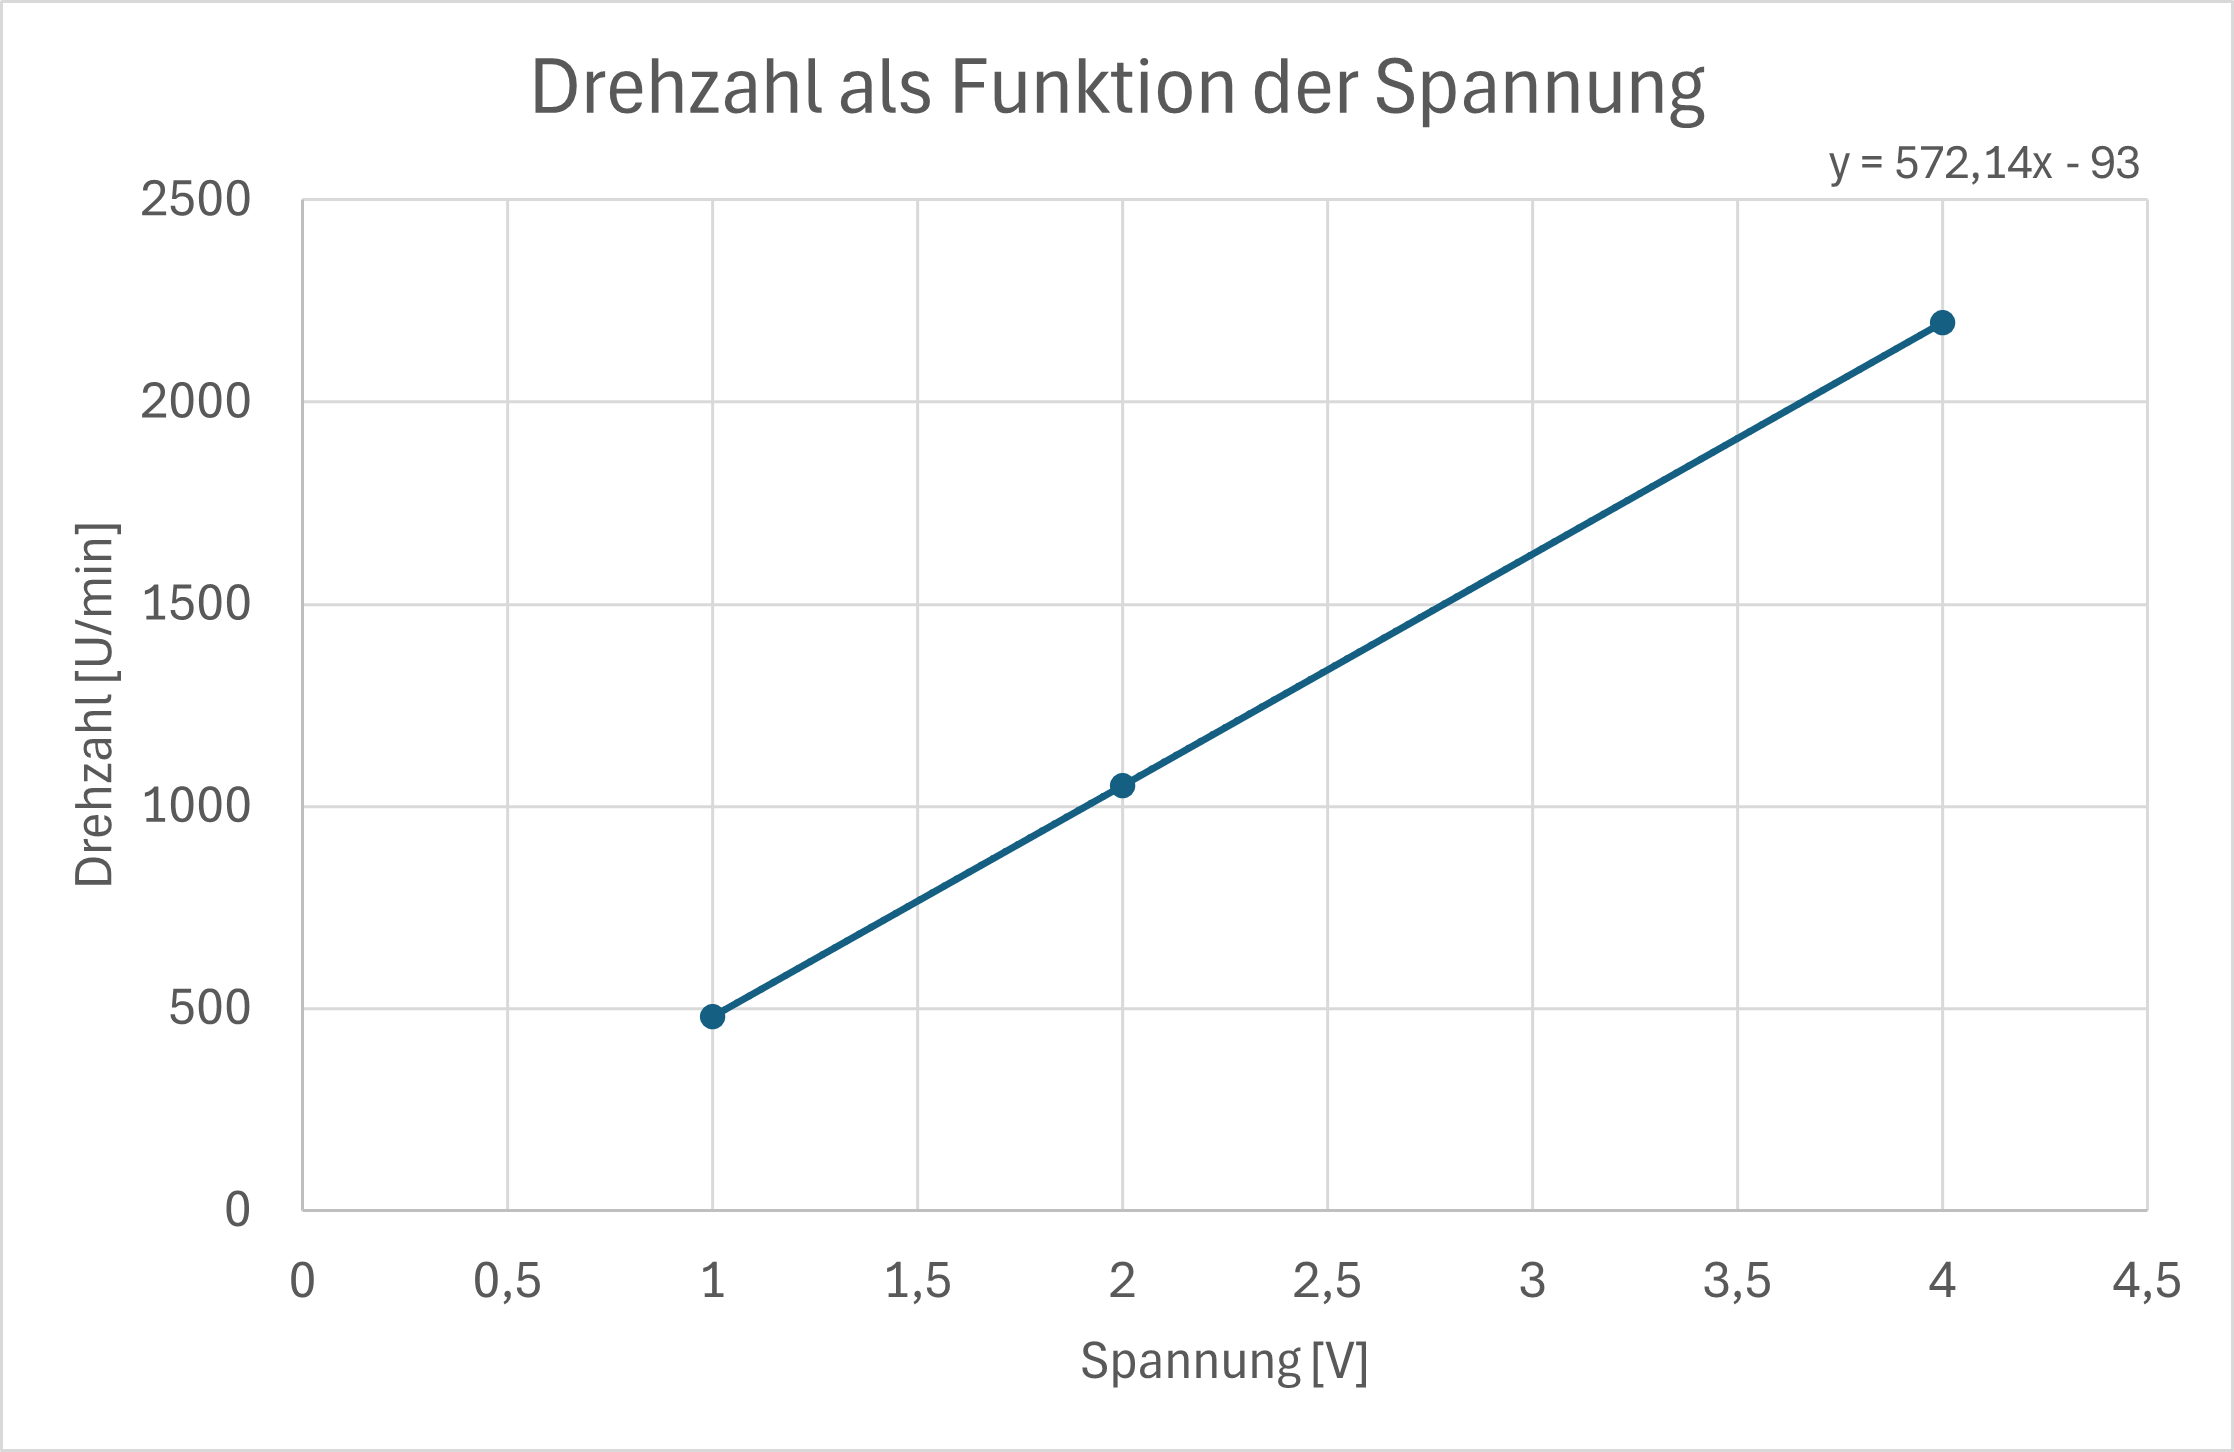
\includegraphics[width=0.7\textwidth]{Drehzahlmessung.png}
        \caption{Zusammenhang zwischen Spannung und Drehzahl}
        \label{fig: Drehzahlmessung}
    \end{figure}

    % Bildbeschreibung
    %-----------------
    \noindent
    Wie in Abbildung \ref{fig: Drehzahlmessung} gut zu sehen ist, verhält sich
    der Zusammenhang zwischen Spannung und Drehzahl wirklich linear. Auch der
    Centerpoint liegt schön auf der Linie. Somit kann folgender Zusammenhang
    angenommen werden:

    % Formel - Zus. zw. Spg. und Drehzahl
    %------------------------------------
    \begin{equation*}
        n = 572.14 \cdot U - 93
    \end{equation*}
%================================================================================

\section{Ergebnisse}
    % Campbell-Diagramm
    %------------------
    Mit den Daten aus den Versuchen kann nun über ein Python-Skript ein
    Campbell-Diagramm erstellt werden (siehe Anhang \ref{sec: Anhang_BSA}). Das
    Skript erstellt für alle 4 Messpunkte ein Diagramm, allerdings wird in der
    Auswertung hier nur Messpunkt 1 (5 rot) betrachet. Das zugehörige
    Campbell-Diagramm ist in Abbildung \ref{fig: Campbell_Diagramm} dargestellt.

    % Bild - Campbell-Diagramm
    %-------------------------
    \begin{figure}[H]
        \centering
        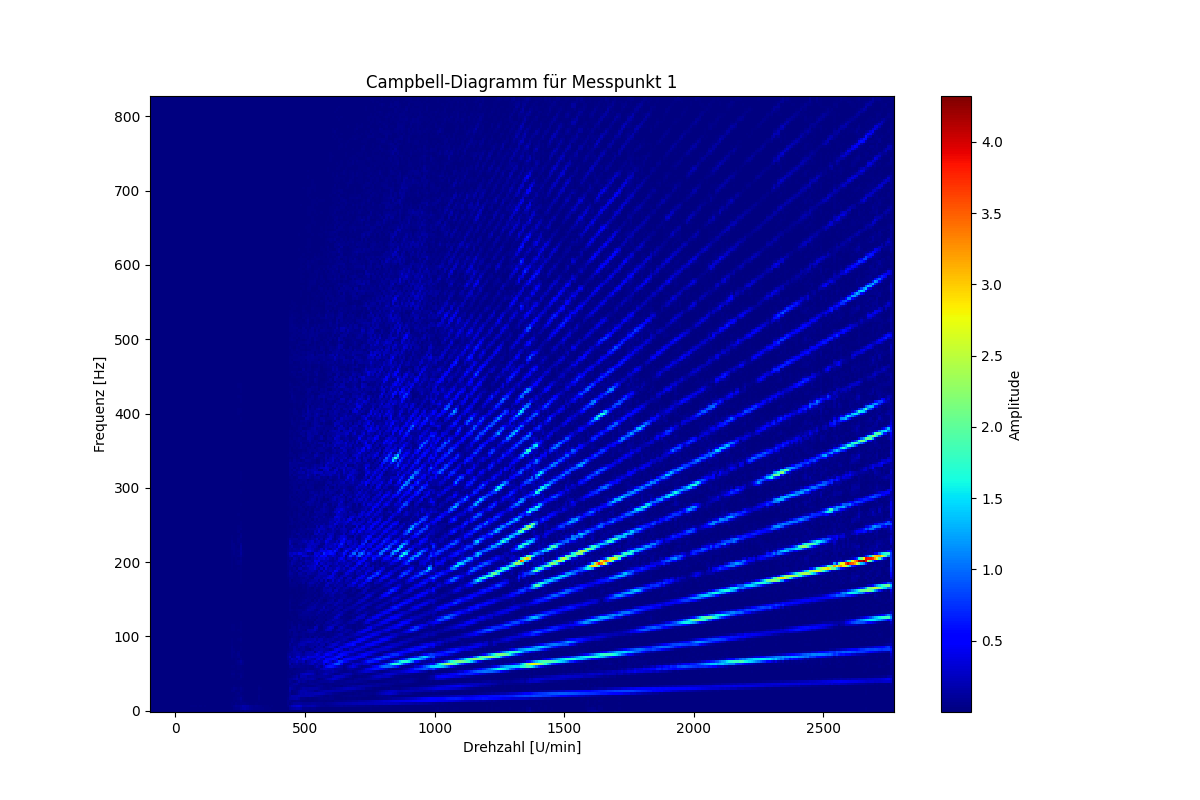
\includegraphics[width=1.2\textwidth]{Campbell_Diagramm_MP1.png}
        \caption{Campbell-Diagramm Messpunkt 1}
        \label{fig: Campbell_Diagramm}
    \end{figure}
    %----------------------------------------------------------------------------

    % Interpretation
    %---------------
    \noindent
    Aus Abbildung \ref{fig: Campbell_Diagramm} geht hervor, dass die meisten der
    Amplitudenausschläge lastabhängig sind. Allerdings sieht es so aus, als ob bei
    etwa 60 [Hz] tatsächlich ein Schwingungsmode liegt. Des Weiteren dürfte auch
    bei zirka 215 [Hz] ein Schwingungsmode liegen. Diese Annahmen decken sich
    auch ganz gut mit dem Amplitudenplot aus Laboraufgabe 1. Wird hier die
    x-Achse weiter angezeigt als bis 60 [Hz], können die beiden oben entdeckten
    Moden auch gesehen werden. Dies ist in Abbildung
    \ref{fig: Modevergleich_CB_EMA} dargestellt.

    % Bild - Modevergleich
    %---------------------
    \begin{figure}[H]
        \centering
        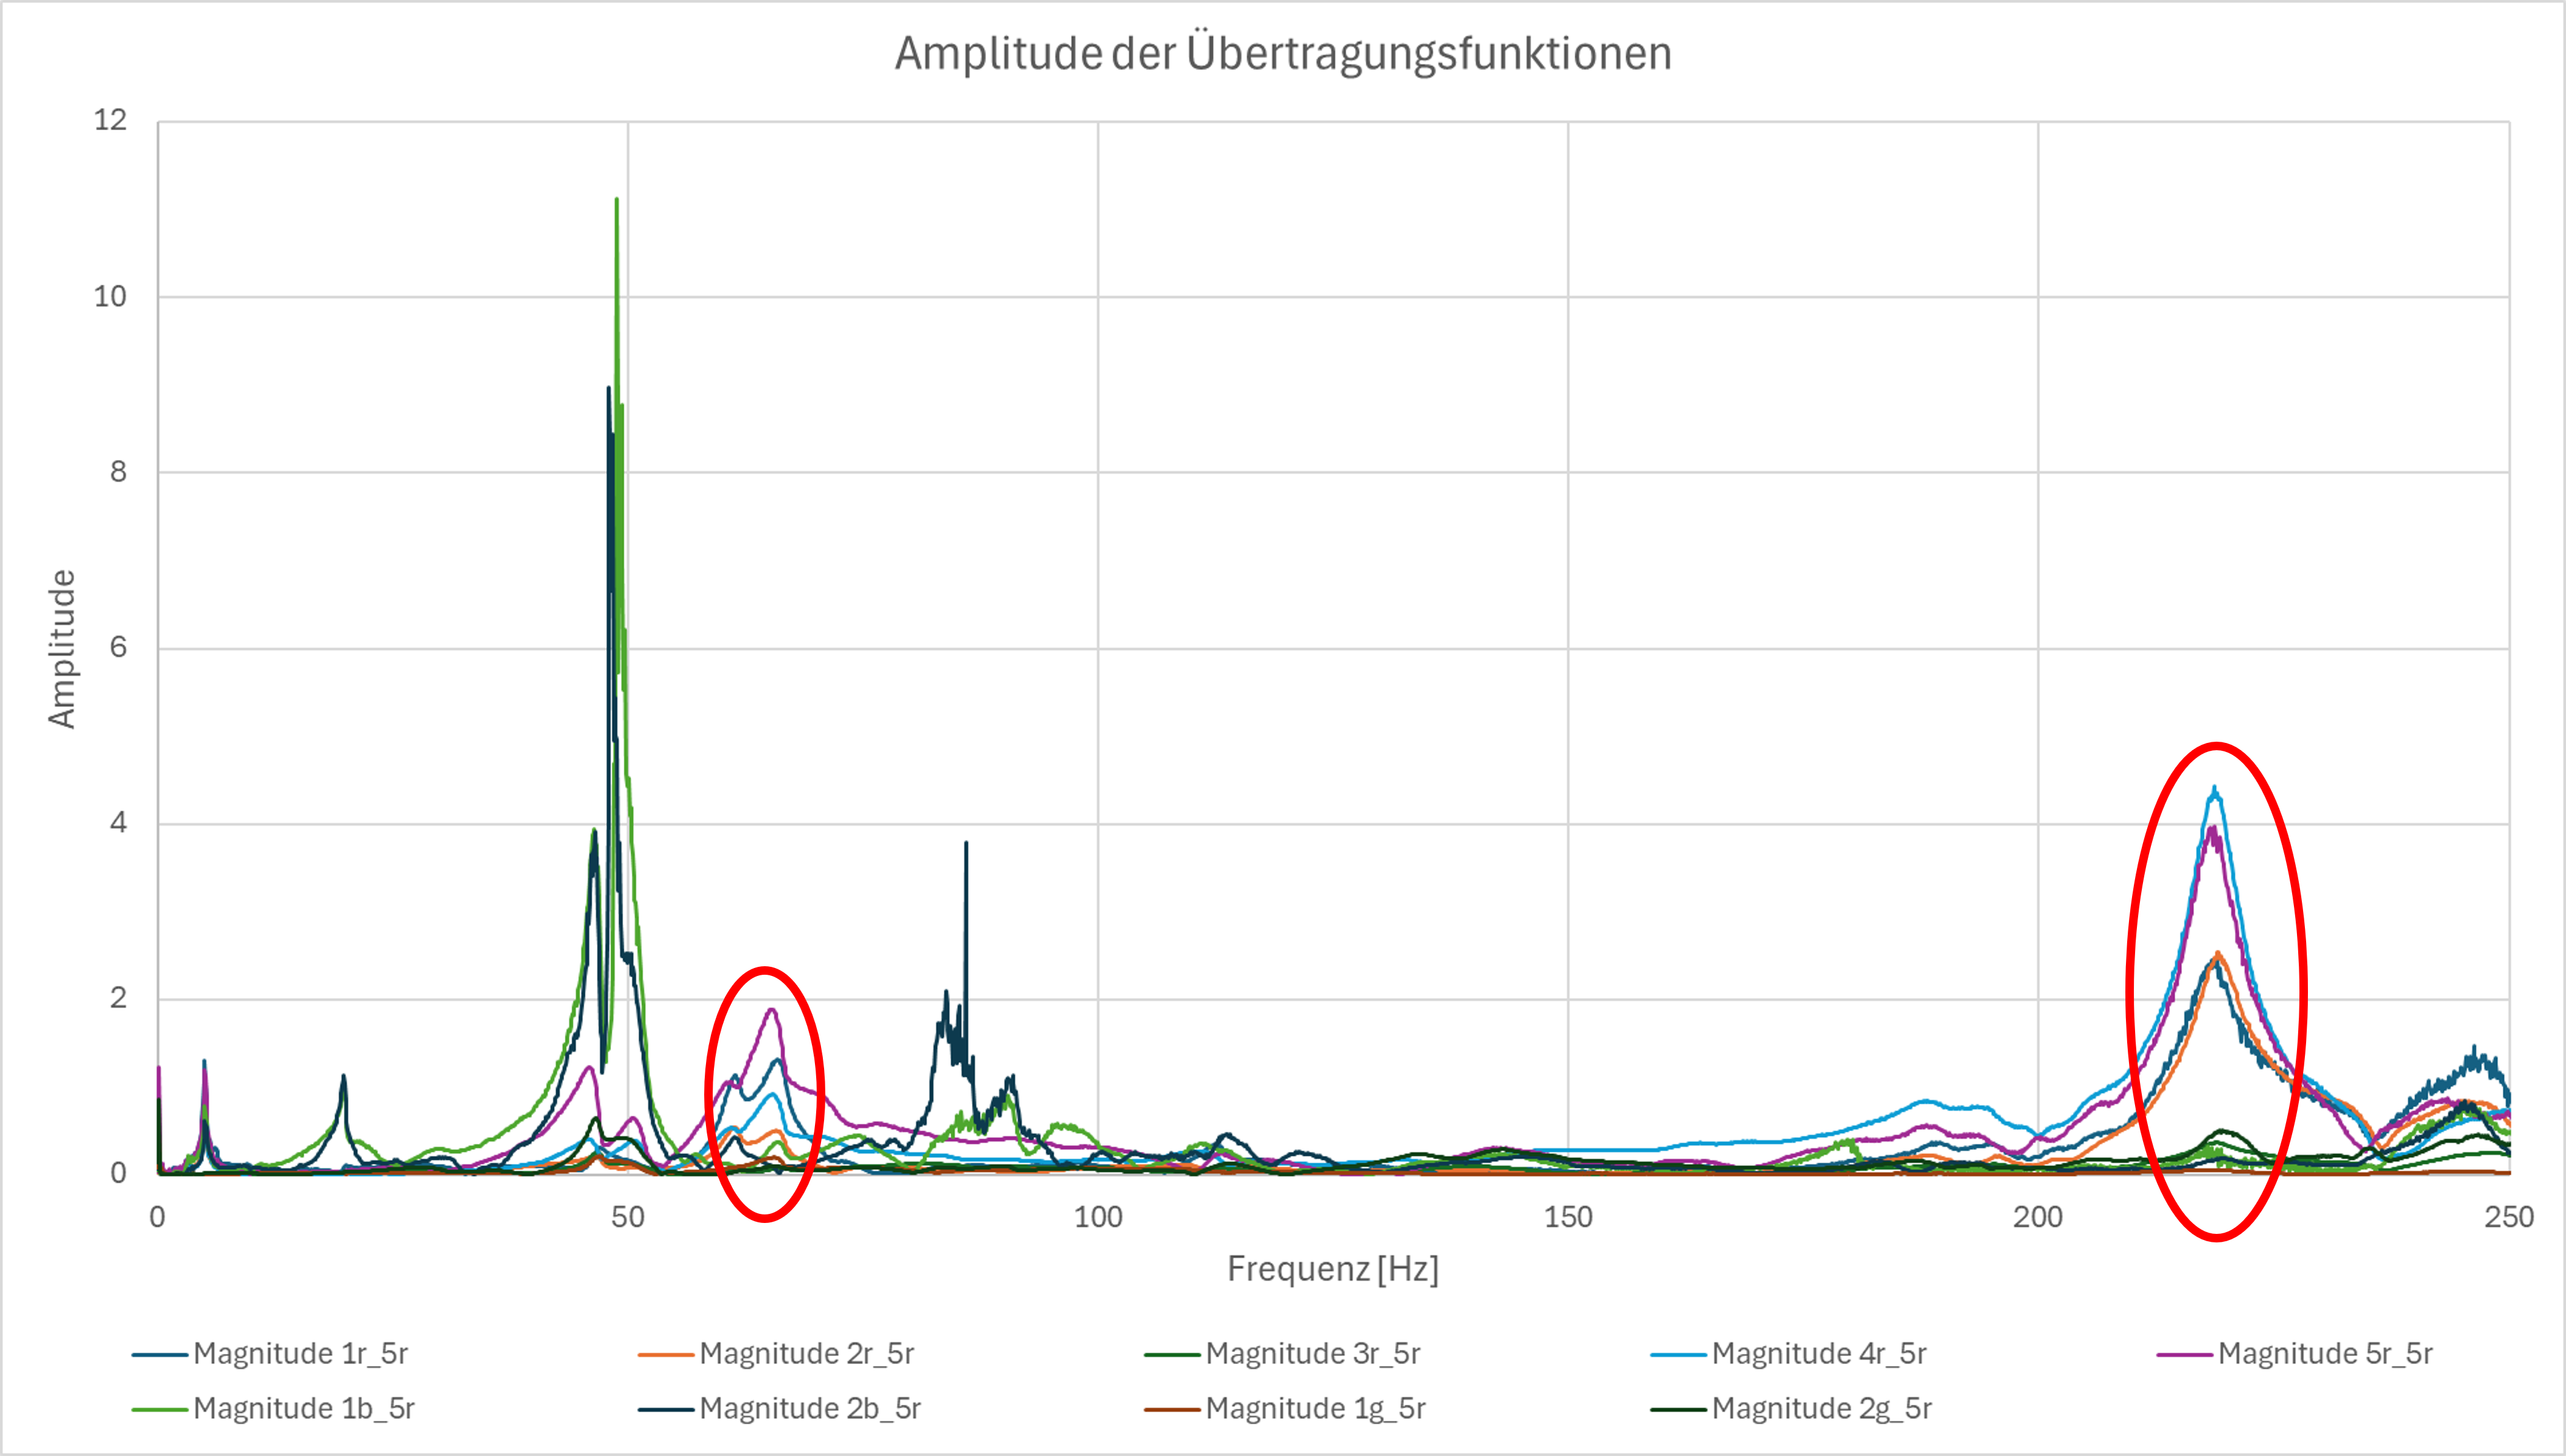
\includegraphics[width=1\textwidth]{Moden_aus_CB_Diagramm.png}
        \caption{Moden des Campbell-Diagramms verglichen mit EMA}
        \label{fig: Modevergleich_CB_EMA}
    \end{figure}



%%----------------------------------------------------------------------------
%% Hauptkapitel 3
	\chapter{Betriebsschwingungsanalyse - HKA}
\label{sec: Hauptkapitel 3}

\section{Aufgabenstellung}
    % Grundziel
    %----------
    Auch bei dieser Laboraufgabe soll eine Betriebsschwingungsanalyse
    durchgeführt werden. Diesmal ist das Zeitsignal jedoch an mehreren, vorher
    definierten, Punkten an der Tragfläche aufzunehmen. Für das Schleppen des
    Motors kann der Versuchsaufbau der vorhergehenden Laborübung verwendet
    werden.
    \\
    %----------------------------------------------------------------------------

    % Ausdetaillierung
    %-----------------
    \noindent
    Nach Aufnahme der Zeitsignale soll eine Hauptkomponentenanalyse (HKA)
    durchgeführt werden. Dies soll einmal für das gesamte Signal gemacht werden.
    In einem 2. Schritt soll die Rampe in 10 gleich große Intervalle unterteilt
    werden. Zu jedem dieser Zeitintervalle gilt es, anschließend eine HKA
    durchzuführen.
%================================================================================

\section{Versuchsaufbau}
%================================================================================

\section{Ergebnisse}
%%----------------------------------------------------------------------------
%% Hauptkapitel 4
	\chapter{DOE - Teilfaktorielle Versuchspläne}
\label{sec: Hauptkapitel 1}

\section{Aufgabenstellung}
%================================================================================

\section{Versuchsaufbau}
%================================================================================

\section{Ergebnisse}
%%----------------------------------------------------------------------------
%% Abbildungsverzeichnis
	\clearpage
	\renewcommand{\listfigurename}{Abbildungsverzeichnis}
\listoffigures
\label{sec: Abbildungen}
\chaptermark{\listfigurename}

%%----------------------------------------------------------------------------
%% Tabellenverzeichnis
\clearpage
\chapter*{Tabellenverzeichnis}
\label{sec: Tabellenverzeichnis}
\addcontentsline{toc}{chapter}{Tabellenverzeichnis}

\listoftables
%%----------------------------------------------------------------------------
%% Anhang
	\clearpage
	\chapter*{Anhang - Python-Code}
\label{sec: Anhang}
\addcontentsline{toc}{chapter}{Anhang - Python-Code}

% Seitennummerierung auf römisch
%===============================
\pagenumbering{Roman}
\appendix

\section{Experimentelle Modalanalyse des Modellflugzeugs}
\label{sec: Anhang_EMA}
%========================================================
    \subsection*{Berechnung\_UeFkt}
    %------------------------------
        \lstinputlisting[language=Python]{Berechnung_UeFkt.py}
        \newpage

    \subsection*{Airplane\_Wireframe}
    %--------------------------------
        \lstinputlisting[language=Python]{Airplane_Wireframe.py}
        \newpage
%%============================================================================	
\end{document}
%%++++++++++++++++++++++++++++++++++++++++++++++++++++++++++++++++++++++++++++
